\newpage
\section{Indexing and Hashing}

\subsection{Basic Concepts}
\begin{enumerate}\small
    \item Indexing mechanisms used to speed up access to desired data.
    \item Search Key - attribute or set of attributes used to look up records in a file.
    \item An index file consists of records (called index entries) of the form: 
    \begin{table}[H]
        \centering
        \begin{tabular}[c]{|c|c|}\hline
            search-key & pointer \\ \hline
        \end{tabular}
    \end{table}
    \item Index files are typically much smaller than the original file.
\end{enumerate}

Two basic $k_i$nds of indices:
\begin{enumerate}
    \item Ordered indices(顺序索引): search keys (index entries) are stored in sorted
    order
    \item Hash indices(散列索引): search keys (index entries) are distributed uniformly across ``buckets'' using a ``hash function''
\end{enumerate}
 3-5

\subsection{Ordered Indices} 7-25

\subsection{\texorpdfstring{$B^+$}.-Tree Index Files}
$B^+$-tree indices are an alternative to indexed- sequential files.
\begin{itemize}\small
    \item Disadvantage of indexed-sequential files
    \subitem Performance degrades as file grows, since many overflow blocks get created.
    \subitem Periodic reorganization of entire file is required.
    \item Advantage of $B^+$-tree index files:
    \subitem Automatically reorganizes itself with\\ small,local,changes, in the face of insertions and deletions.
    \subitem Reorganization of entire file is not required to maintain performance.
    \item (Minor) disadvantage of $B^+$-trees:
    \subitem Extra insertion and deletion overhead; space overhead.
    \item Advantages of $B^+$-trees outweigh disadvantages
    \subitem $B^+$-trees are used extensively
\end{itemize}

\begin{figure}[!htb]
    \centering
    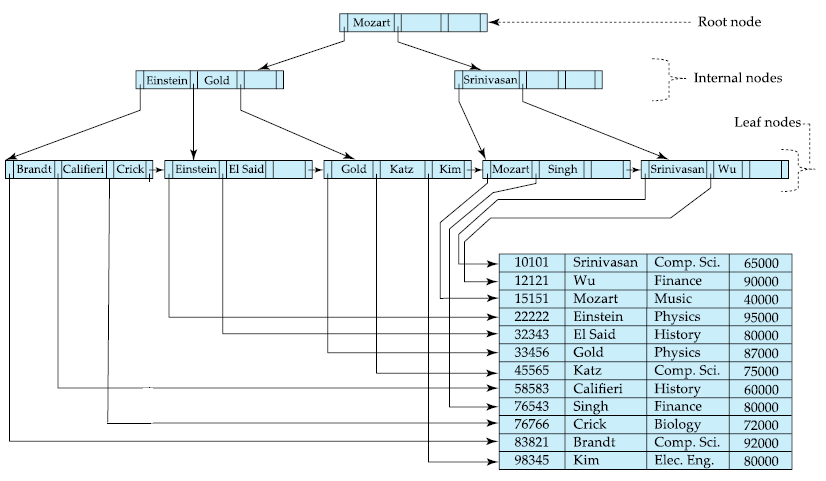
\includegraphics[width=0.42\textwidth]{DB8/Example of B+-Tree}
    \caption{Example of $B^+$-Tree}
\end{figure}

A $B^+$-tree is a rooted tree satisfying the following properties: 
\begin{enumerate}\small
    \item All paths from root to leaf are of the same length –-- balanced tree
    \item Each node that is not a root or a leaf has between $\left\lceil \frac{n}{2} \right\rceil$ and $n$ children.
    \item A leaf node has between $\left\lceil \frac{n-1}{2} \right\rceil$ and $n–1$ values
    \item Special cases:
    \subitem If the root is not a leaf, it has at least 2 children.
    \subitem If the root is a leaf (that is, there are no other nodes in the tree), it can have between 0 and $(n–1)$ values.
\end{enumerate}

\subsubsection{\texorpdfstring{$B^+$}.-Tree Node Structure}
%TOOD P30
\begin{figure}[!htb]
    \centering
    \begin{tikzpicture}
        
    \end{tikzpicture}
    \caption{Typical node}
\end{figure}

\begin{itemize}
    \item $K_i$ are the search-key values
    \item $P_i$ are pointers to children (for non-leaf nodes) or pointers to records or buckets of records (for leaf nodes)
    \item 通常,一个节点对应一个block
\end{itemize}
The search-keys in a node are ordered
\begin{align*}
    K_1 < K_2 <\dots <K_{n-1}
\end{align*}
(Initially assume no duplicate keys, address duplicates later)

\subsubsection{Leaf Nodes in \texorpdfstring{$B^+$}.-Trees}
For $i = 1, 2, \dots, n–1$, pointer $P_i$ either points to a file record with search-key value $K_i$, or to a bucket of pointers to file records, each record having search-key value $K_i$. Only need bucket structure if search-key does not form a primary key. (like dense index, every search key appears in leaf nodes)
 P31

\subsubsection{Non-Leaf Nodes in \texorpdfstring{$B^+$}.-Trees}
 P32


\subsubsection{Queries on \texorpdfstring{$B^+$}.-Trees}
 P35-36

\subsubsection{Handling Duplicates}
 P37

\subsubsection{Updates on \texorpdfstring{$B^+$}.-Trees: Insertion}
 P38-42

\subsubsection{Updates on \texorpdfstring{$B^+$}.-Trees: Deletion}
 P43-47

\subsubsection{Non-Unique Search Keys}
 P53

\subsubsection{B+-Tree File Organization}
 P54


\subsection{Write-optimized Indices}

\subsubsection{Log Structured Merge (LSM) Tree}
 P82

\subsubsection{Buffer Tree}
 P85

\subsection{Index Definition in SQL}
 P86